%!TEX TS-program = pdfLaTeX
%!TEX encoding = utf-8
%!TEX spellcheck = fr-FR

\documentclass[12pt,twoside,openright]{article}

%nœud

%\usepackage{soul}

%\documentclass[a4paper,11pt]{book}
\usepackage[T1]{fontenc}
\usepackage[utf8]{inputenc}
\usepackage[francais]{babel}

\usepackage[usenames,dvipsnames]{color}

\usepackage{lmodern}
%%%%%%%%%%%%%%%%%%%%%%%%%%%%%%%%%%%%%%%%%%%%%%%%%%%%%%%%%
% Source: http://en.wikibooks.org/wiki/LaTeX/Hyperlinks %
%%%%%%%%%%%%%%%%%%%%%%%%%%%%%%%%%%%%%%%%%%%%%%%%%%%%%%%%%
\usepackage{hyperref}
\usepackage{graphicx}
\usepackage{pdfpages}
\usepackage{amsmath}
\usepackage{amssymb}
\usepackage{a4}
\usepackage{indentfirst}
\usepackage{fancyhdr}
\usepackage{varioref}
\usepackage{makeidx}

%\usepackage{biblatex}
\usepackage{mslapa}

\usepackage[normalem]{ulem}



%% Apalike hyphenation %%%
%\let\oldbibitem=\bibitem
%\renewcommand{\bibitem}[2][]{\oldbibitem[#1]{#2}\newline}

%%% Margins %%%
\voffset -2.54cm
\textheight 24cm
\hoffset -1.3in
\evensidemargin 2.5cm
\oddsidemargin 2.5cm
\textwidth 18cm

% Book's title and subtitle
\title{\textbf{Toward Predictive Machine Learning for Active Vision} }
% Author
\author{\textsc{Emmanuel Daucé}}%\thanks{\url{www.example.com}}}
\date{}
\makeindex

\begin{document}
	
\maketitle
	
	The oculo-motor activity is an essential component of man and animal behavior, subserving most of daily displacements and interactions with objects, devices or people. By moving gaze with the eyes, the center of sight is constantly and actively moving around during all waking time.  %Though taking a large part in brain activity, the principles underlying those visually guided movements are still a subject of debate in neurosciences.
	The {\it active vision paradigm}~\cite{friston2012perceptions}, recently developed in neuroscience, relies on a longstanding history of probabilistic modelling in signal processing and control \cite{Kalman1960,Baum1966,friston1994statistical}. 
	It considers an organization of the visual space in objects (or causes), whose presence and position is continuously checked by visual inspection. For instance, saccades are considered in this theory to be probing a particular region of the visual space, with the objective of reducing the uncertainty about the identity and position of particular objects. %This theory takes for granted that an a priori knowledge exists on all possible objects and locations but also for the repertoire of movements.
	
	Put formally, exploring a visual scene through saccades consists in identifying objects in space through the foveation of parts of the scene only. The cause of the current visual field $y$ is both the object identity $o$, its position in the peripersonal space $x$, and the current visual orientation $u$, i.e. $y \sim P(Y|x,o,u)$, each variable counting for a distinct degree of freedom. % and the generative process  for every possible composition of object identity $o \in \mathcal{O}$, position $x \in \mathcal{X}$ and $u \in \mathcal{U}$. 
	In a model-based approach, with $P$ the generative process, the active vision paradigm mainly considers optimizing the choice of $u$ for reducing uncertainty about $x$ and $o$, which are the undisclosed constituents of the scene. For simplicity $x$ and $o$ are here reduced to a single variable $z = (x, o)$. Considering now that a certain prior $\pi(z)$ has been formed about $z$, choosing  $u$ conducts the sight in a region of the visual field that provides $y$, which in turn allows to refine the expectations about the cause of the perception, i.e.
	$ P(z|u,y) \propto P(y|z,u) \pi(z)$. 
	One needs thus to choose $u$ appropriately in order to reduce the uncertainty about $z$, given the actual $y$, i.e minimize the entropy :
	$u^* = \underset{u \in \mathcal{U}}{\text{argmin }} H$ with $H = E(-\log P(z|u,y))$.
	
	This optimal $u$ is not known in advance, because $y$ is only read \emph{after} $u$ has been carried out. Then comes the predictive framework that identifies the effect of $u$ with its most probable outcome, according to the predictive model. This can for instance be done under a greedy setup, i.e. first set $\tilde{z} = \underset{z \in \mathcal{Z}}{\text{argmax }} \pi(z)$, second set $\forall u, \tilde{y}_u = \underset{y \in \mathcal{Y}}{\text{argmax }} P(y|\tilde{z},u)$.
	Finally, set 
	\begin{equation}
	\tilde{u} = \underset{u \in \mathcal{U}}{\text{argmax }}  P(\tilde{z}|u,\tilde{y}_u))
	\end{equation} which is a proxy for minimizing the entropy. This greedy choice tells in short that if $\tilde{z}$ is the running hypothesis, the operator should orientate his sight toward 
	%the part of the scene where he thinks his assumption should receive confirmation, i.e. 
	the part of the scene that is the most discriminative toward confirming $\tilde{z}$ against all other possibilities. 
	
	This series of operations can be repeated in a sequence, where the visual orientation $\tilde{u}$ is followed by reading the effective visual field $y$, allowing to update the priors about the cause of perception, i.e. $\forall z, \pi'(z) \propto  P(y|z,\tilde{u}) \pi(z)$. In that framework, saccadic exploration means thus to define a sequence of visuo-motor commands $\tilde{u}$, $\tilde{u}'$, $\tilde{u}''$, ... This sequence should ultimately provide a final estimate $\pi^{(n)}(z)$ such that a single cause $\hat{z}$ may dominate the other ones, allowing the system to reach a final decision.   
	
	For illustrative purpose, this setup was tested on a classic machine learning image processing setup, namely the MNIST dataset. In order to mimic a foveated exploration, a 2D-wavelet decomposition is performed on the images, providing a series of triplets of wavelet coefficients organized in space and in different levels. A visual orientation command $u = (i,j)$ then allows to read out several wavelets coefficient triplets associated with the considered coordinate (at different levels). Given a model $P(y|u,z)$, each  wavelet coefficients triplet $y$ is thus expected to participate in uncovering the underlying object $z$ (here a digit between 0 and 9).

	\begin{figure}[t!]
		\centerline{
				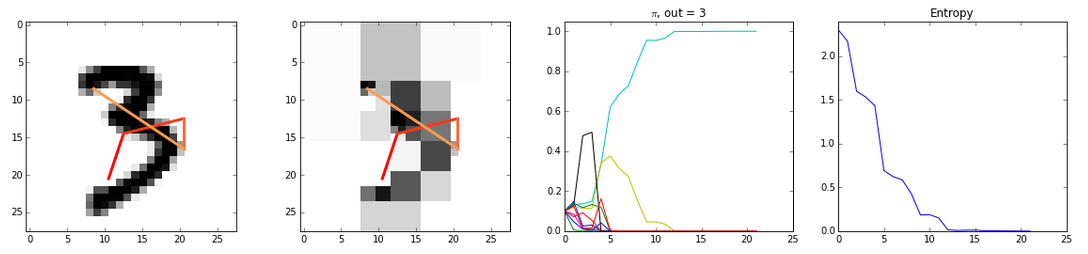
\includegraphics[width = \linewidth]{figure.png} 
		}
		\centerline{\bf a \hspace{4cm} b \hspace{4cm} c \hspace{4cm} d}
		\caption{\footnotesize{{\bf Saccadic exploration for digit image recognition}~. {\bf a.} Saccades trajectory (from red to orange) superimposed over an original digit. {\bf b.} Saccades trajectory over reconstructed image from available visual information. {\bf c.} Posterior probability update, in function of the number of wavelet triplets observed. {\bf d.} Entropy of the posterior, in function of the number of wavelet triplets observed. } }
	\end{figure}
	
	The predictive model is built on a 55,000 example set, and reaches approximately 92 \% correct recognition on the test set. The image decomposition in a dictionary of wavelets coefficients is rather rough, though providing a simple validation of the proposed setup. The performance is also quite satisfying given the model lightness, when compared to hard-working layered dictionary construction in convolutional neural networks. 
	More importantly, the decision over the predicted posterior (eq. 1), that scans all possible outcomes of actions, can be pre-processed and stored in a table to simplify decision. The structure of the decision process is moreover consistent with the reinforcement and online learning frameworks, with action outcome possibly assimilated with the (log)-likelihood of the visual field, and/or with higher level target reaching/achievement criterions.
	
	{\color{magenta} The artificial curiosity framework posits that the part of the visual scene being the less congruent with the current assumption should attract visual attention. Choosing the part of the scene with the highest discriminative power maximises the chance to find the visual input sur
		
		where the chance to find a non-congruent visual input is the highest, i.e.
		$$ \underset{u}{\text{argmin }} P(y|z,u) P(z)$$
		This idea 
		Regarding the artificial curiosity thematic, the model presented her posits that the model is attracted by regions of the visual field that should maximize the surprise if the current assumption is wrong}
	
	This account of image recognition through saccades links to the case of a living system having to react at sort notice in a complex environment with limited resources. Some critical signals need to be interpreted fast, and many others need to be ignored. Not all the visual surroundings need to be scanned, but only the critical features, shapes and displacements. This is the essence of visual orientation, and our hypothesis is that efficient object-specific saccade sequences may be pre-learned to facilitate recognition under prior assumptions about the state of the environment. 
	
	%How robust and efficient such decision making is achieved is not only important for neuroscience, but also for robotics, which faces similar constraints.   %both topics, both at the level of each objective  but also globally. %However, a property of the generic systems we propose is that they should 
	%As such, it is necessary to extend this problem to a generic set of conditions which are relevant to the trajectory of objects' contours in natural scenes, that is, for different configurations of the scene such as the presence of different types of objects.
	
	%Taking guidance from the biological observations, the idea is to consider the natural strategies adopted to deal with limited sensors and limited computing resources.
	%: how use at best low sensory bitrate and noisy sensors? how much memory use, what motor decisions make to maintain a consistent model of the outside scene? 
\begin{footnotesize}
\bibliographystyle{apalike}
\bibliography{biblio}
\end{footnotesize}	
	
\end{document}